%
% File: chap02.tex
% Author:
% Description: Background
%
\chapter{Background}
\label{chap:background}

% Description

\section{Relative Work}
\label{sec:relative-work}


In South Africa, both large public hospitals and primary healthcare (PHC) facilities are under heavy pressure. Large hospitals are often overcrowded because of the high number of patients. Many PHC clinics are also not in good condition. A study reported that 83\% of patients had to wait for a long time before they could see a healthcare worker, mainly because of a lack of staff, outdated facilities, shortage of medicines, and low administrative efficiency \cite{nwagbara2024}.

In our project, we try to improve this situation through the Smart Hospital System in two main ways. First, it provides online consultations and a Health Q\&A platform, so that patients can get medical advice from home without going to already crowded hospitals or PHC facilities. Second, it works with local clinics to provide regular vital sign measurements such as blood pressure, heart rate, and blood glucose checks to help with chronic disease monitoring. By doing so, many routine check-ups do not need to be done at large hospitals, which can reduce crowds and also allow small clinics to do more things for the local hospital.

Actually, South Africa has already started to use digital health methods to deal with the shortage of healthcare resources. Research has shown that telemedicine is being used for chronic disease management and mental health care, but there are still challenges with policies and the digital divide \cite{agbeyangi2025}. Other studies also show that telemedicine can reduce transportation and cost barriers, making chronic care easier to get \cite{sayani2019}.

The goal of this project follows the United Nations Sustainable Development Goal (SDG) 3, ``Ensure healthy lives and promote well-being for all at all ages'' \cite{sdg3}. It also matches South Africa's National Development Plan 2030, which talks about reducing waiting times in public healthcare facilities \cite{ndp2030guideline}.

\section{Existing Solutions}
\label{sec:existing-solutions}

Although our system is designed for South Africa, we also looked at existing online healthcare solutions globally to get ideas for features and understand what works well and what could be improved.

\subsection{Teladoc Health}
Teladoc Health is a popular online medical platform \cite{teladocwebsite} that offers services like video calls with doctors and support for mental health. It is used in many countries and is helpful for people who find it hard to go to a hospital.

\begin{figure}[htbp]
    \centering
    \begin{minipage}[b]{0.47\textwidth}
        \centering
        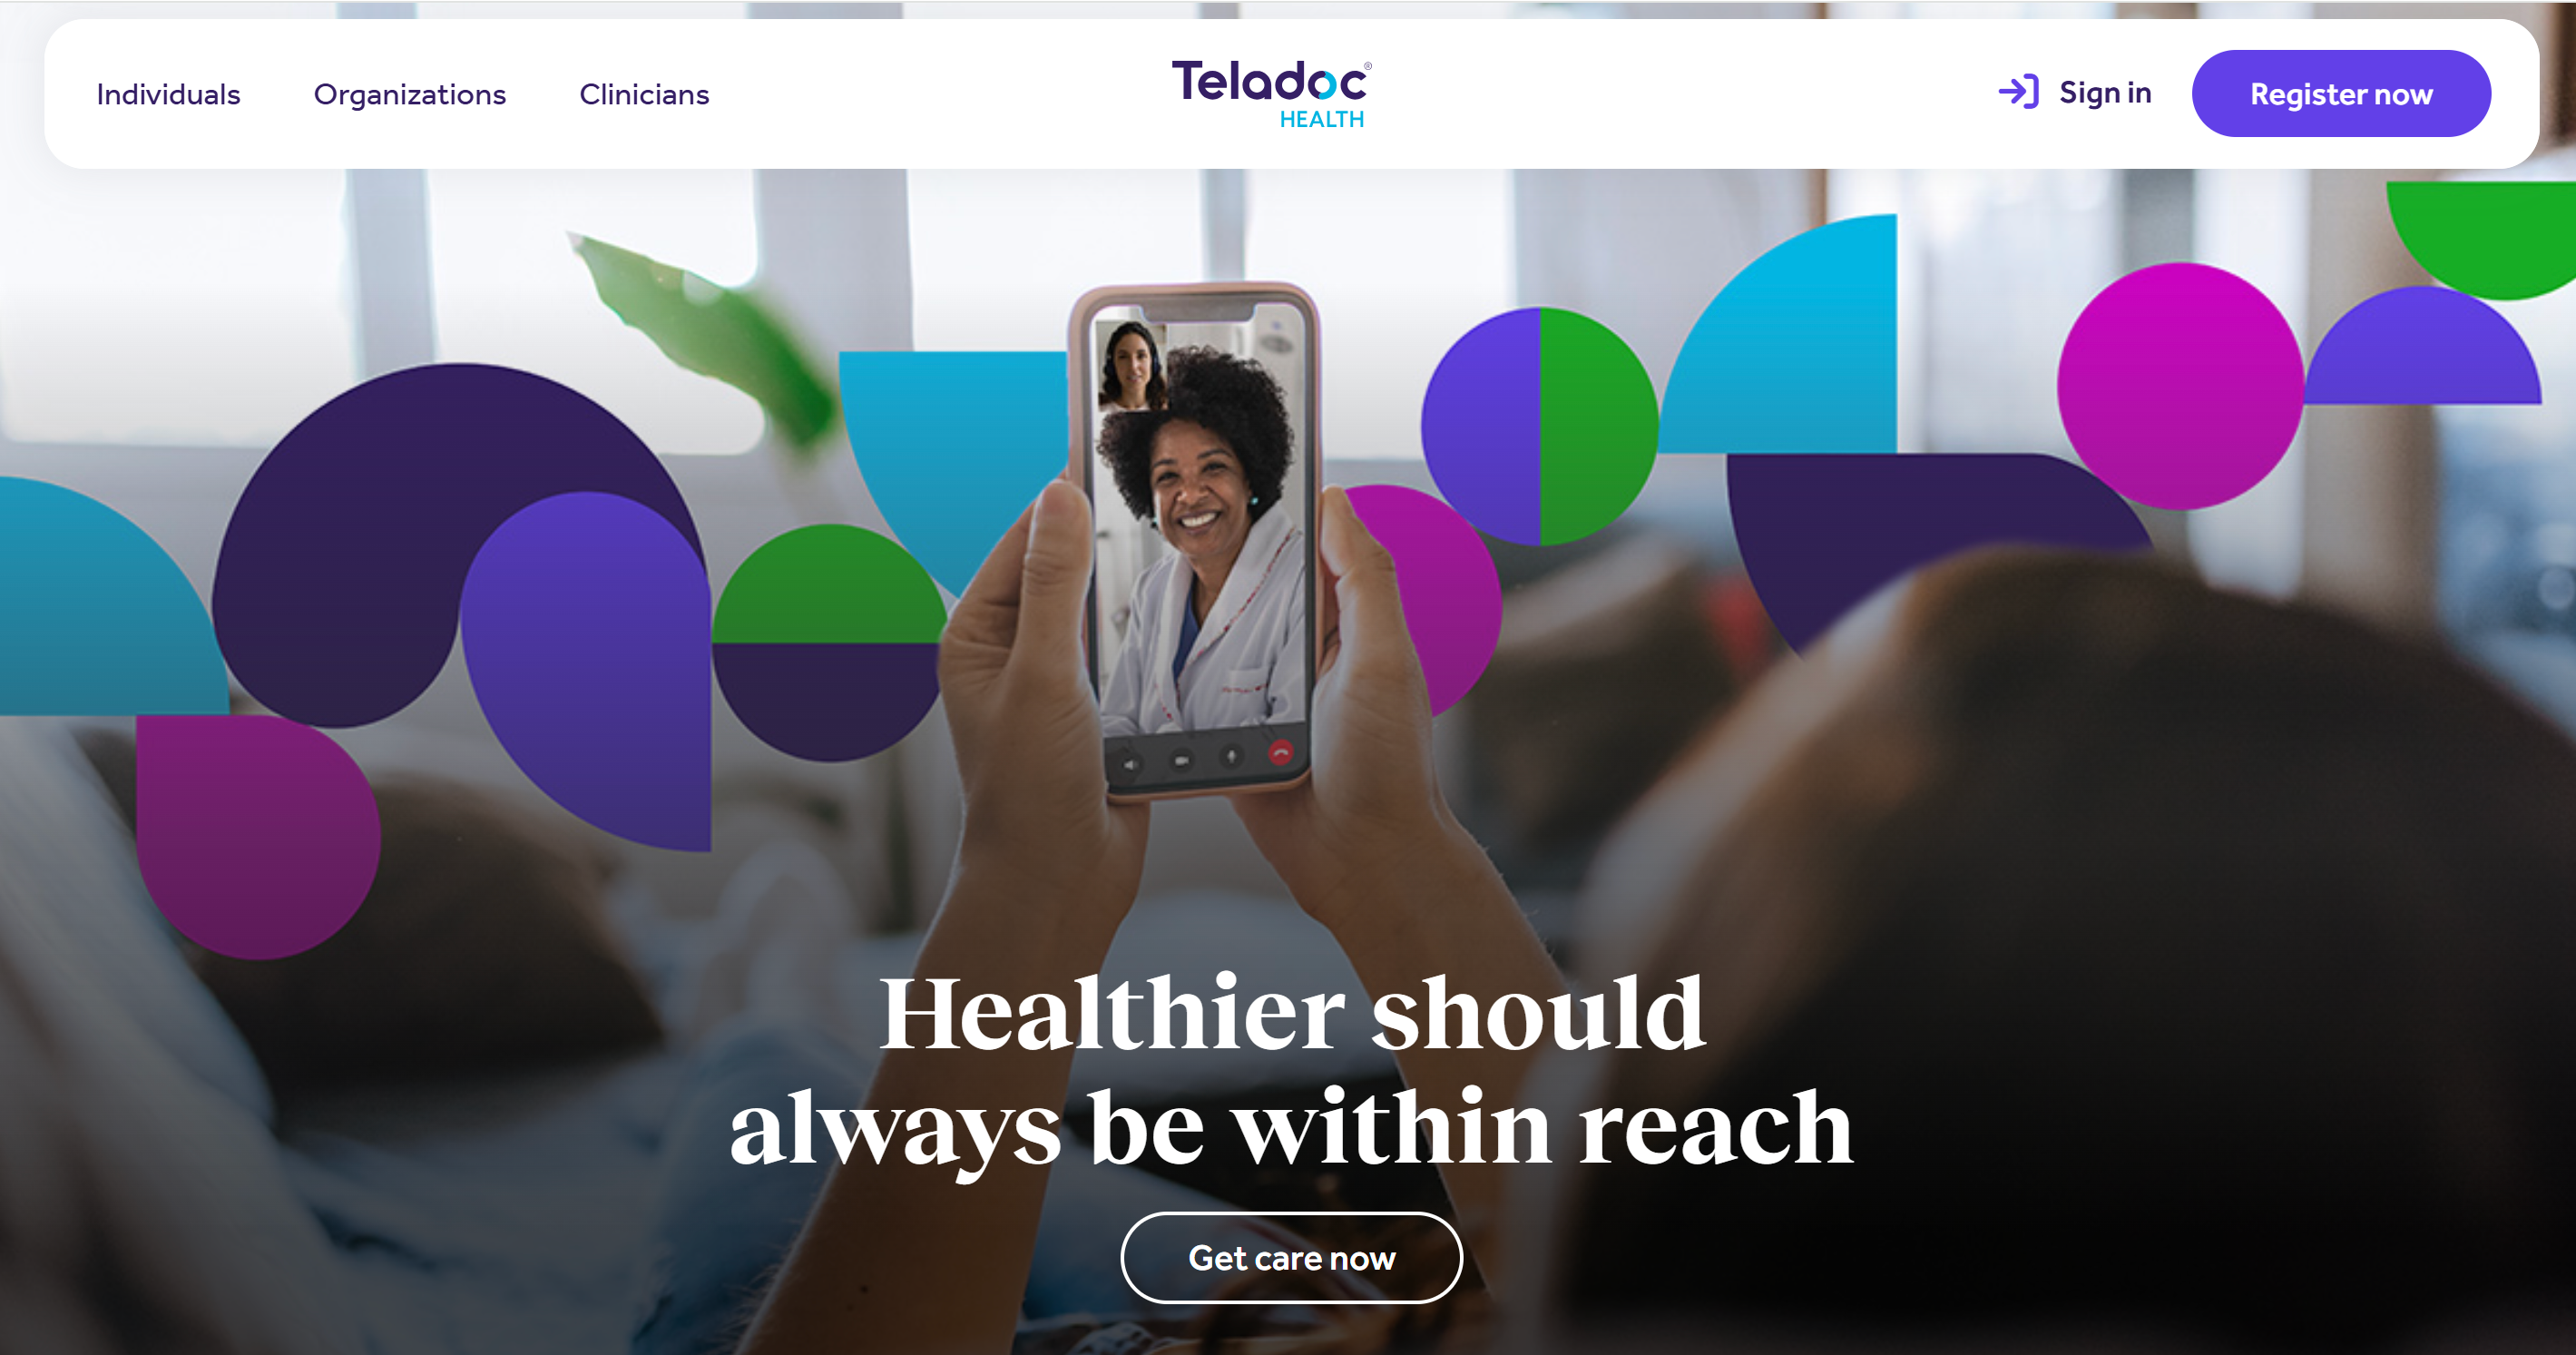
\includegraphics[width=\textwidth]{../../images/telodocHome.png}
        \caption{Homepage of Teladoc Health.}
        \label{fig:teladoc-home}
    \end{minipage}
    \hfill
    \begin{minipage}[b]{0.47\textwidth}
        \centering
        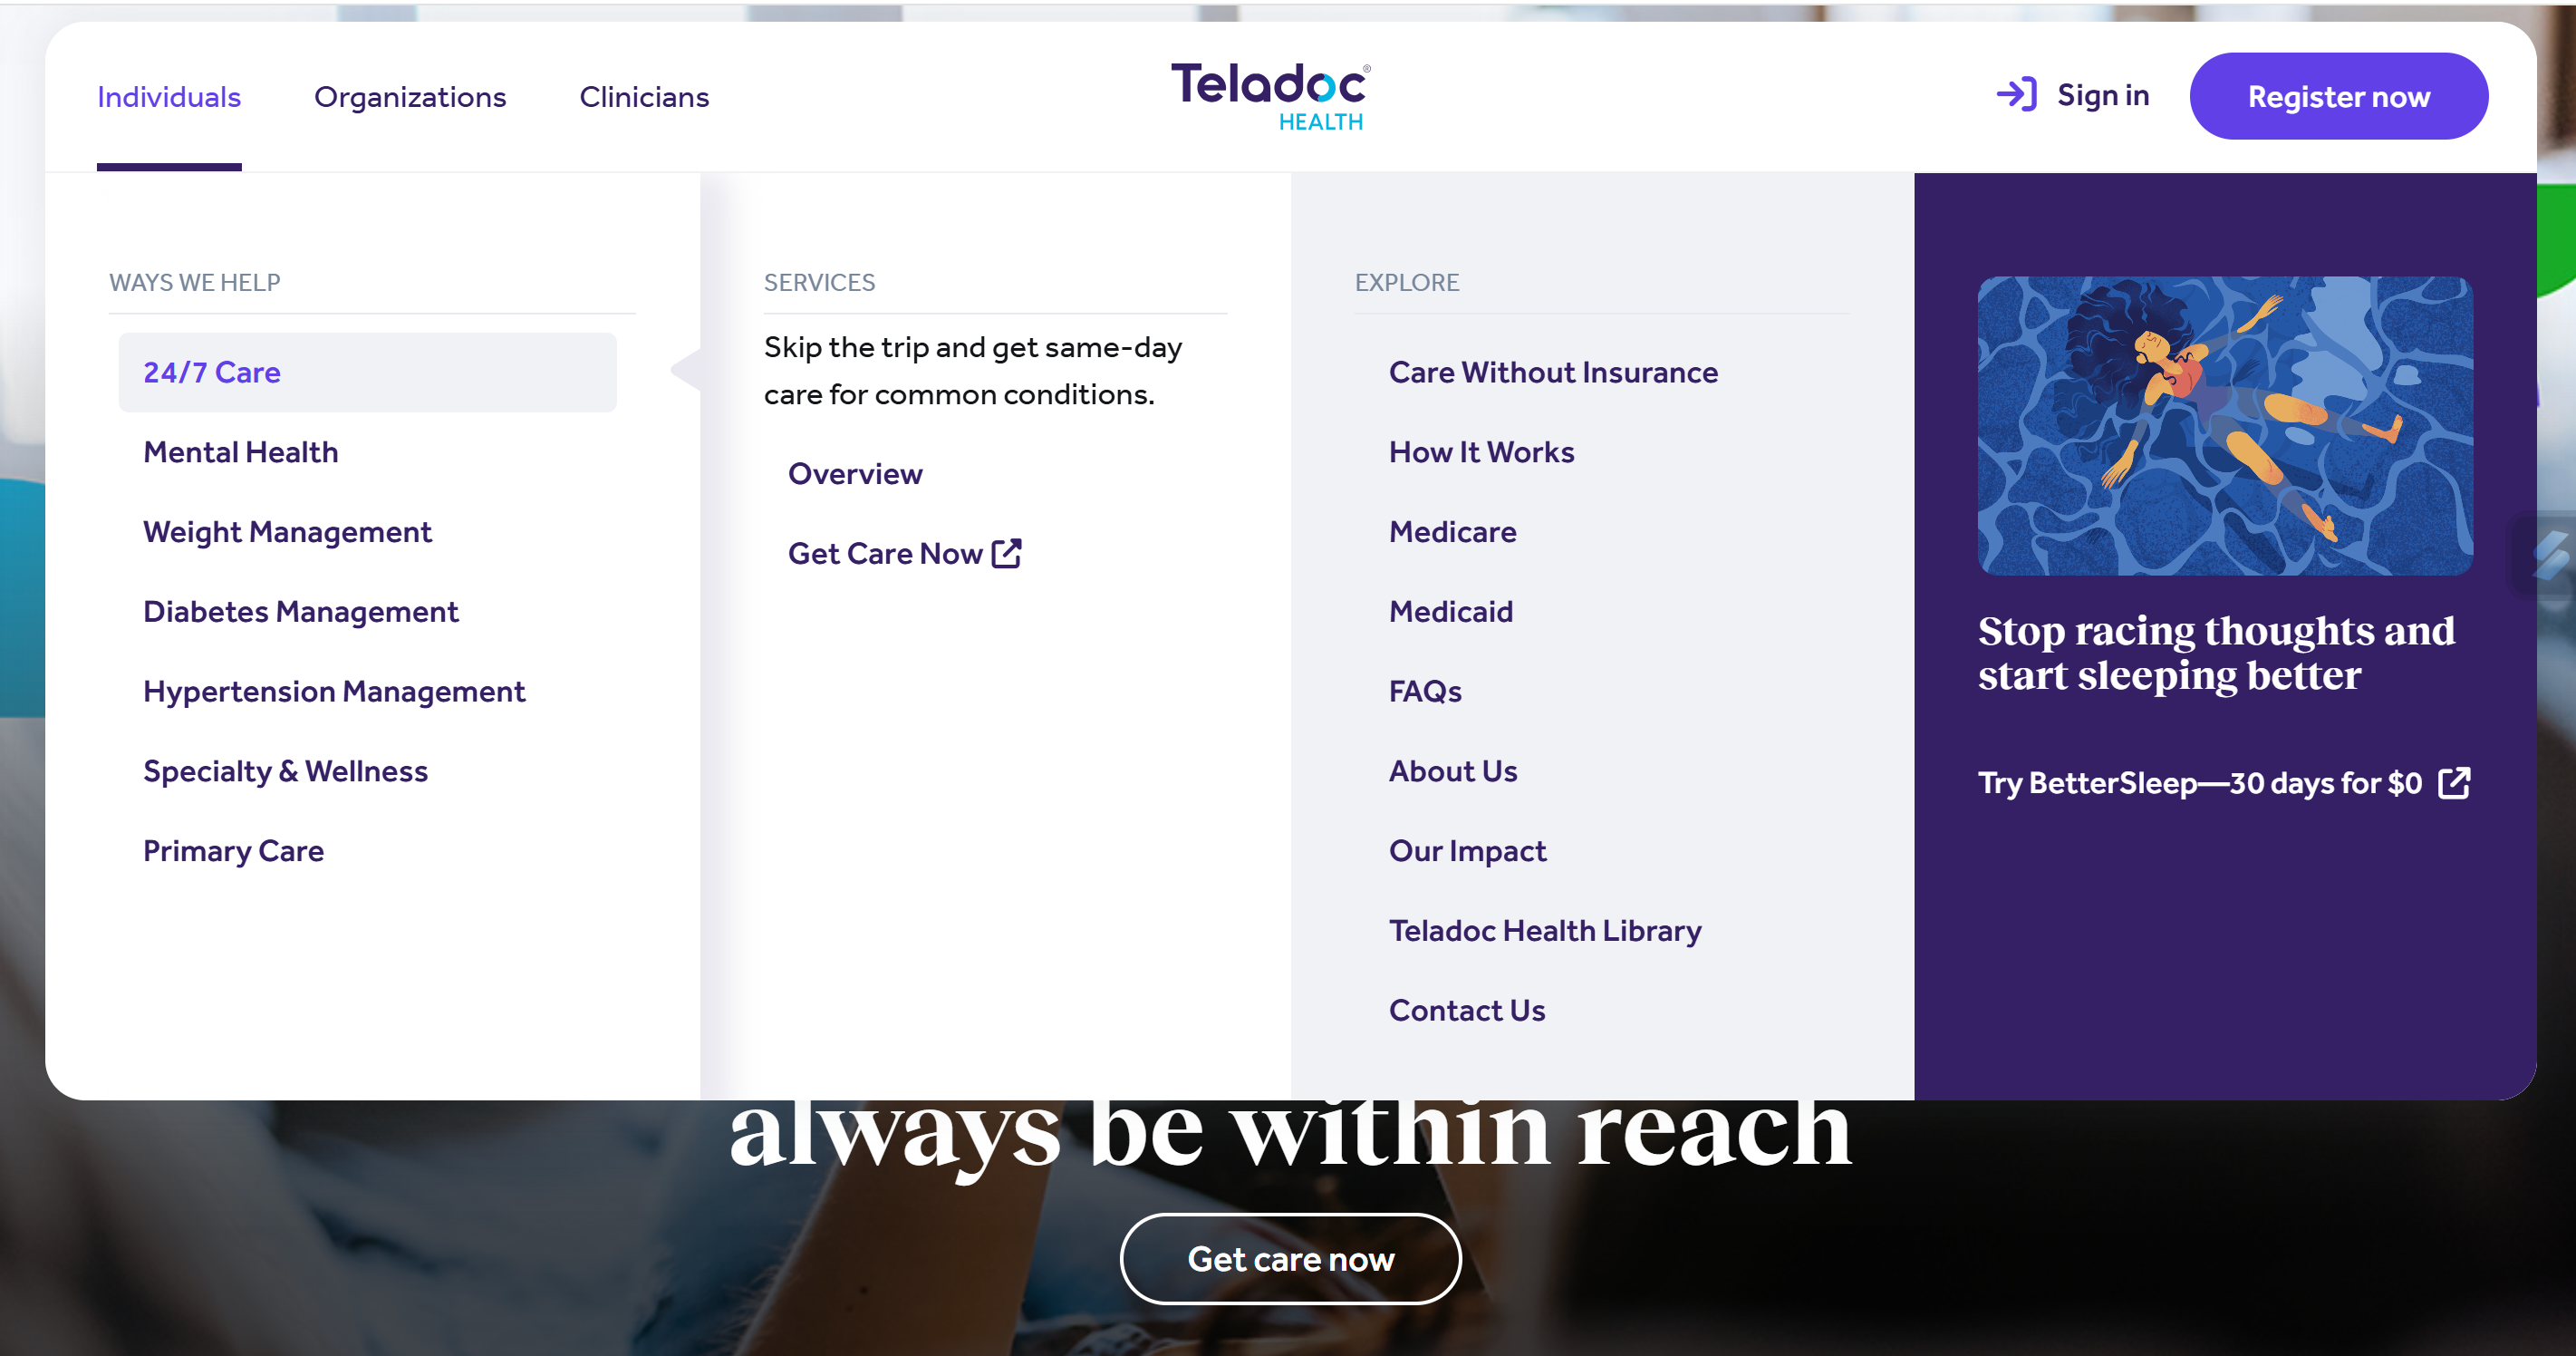
\includegraphics[width=\textwidth]{../../images/telodocServices.png}
        \caption{Service menu of Teladoc Health.}
        \label{fig:teladoc-services}
    \end{minipage}
\end{figure}

However, there are still some problems, especially for South Africa. For example, people with chronic diseases still need to go to hospitals to do regular vital checks, so they still have to wait for a long time. Also, Teladoc usually needs subscription or pay-per-use, which can be too expensive for people in low-income areas.

\subsection{LINE Hospital Services}

In Taiwan, many hospitals have their own official LINE accounts to provide online services. Patients can add the hospital’s LINE to do things like online appointment booking and checking doctor information and hospital outpatient schedules. It is very easy to use because most people in Taiwan already use LINE every day. In South Africa, it may be WhatsApp instead.

\begin{figure}[H]
    \centering
    % left with chinese
    \begin{subfigure}[t]{0.3\textwidth}
        \centering
        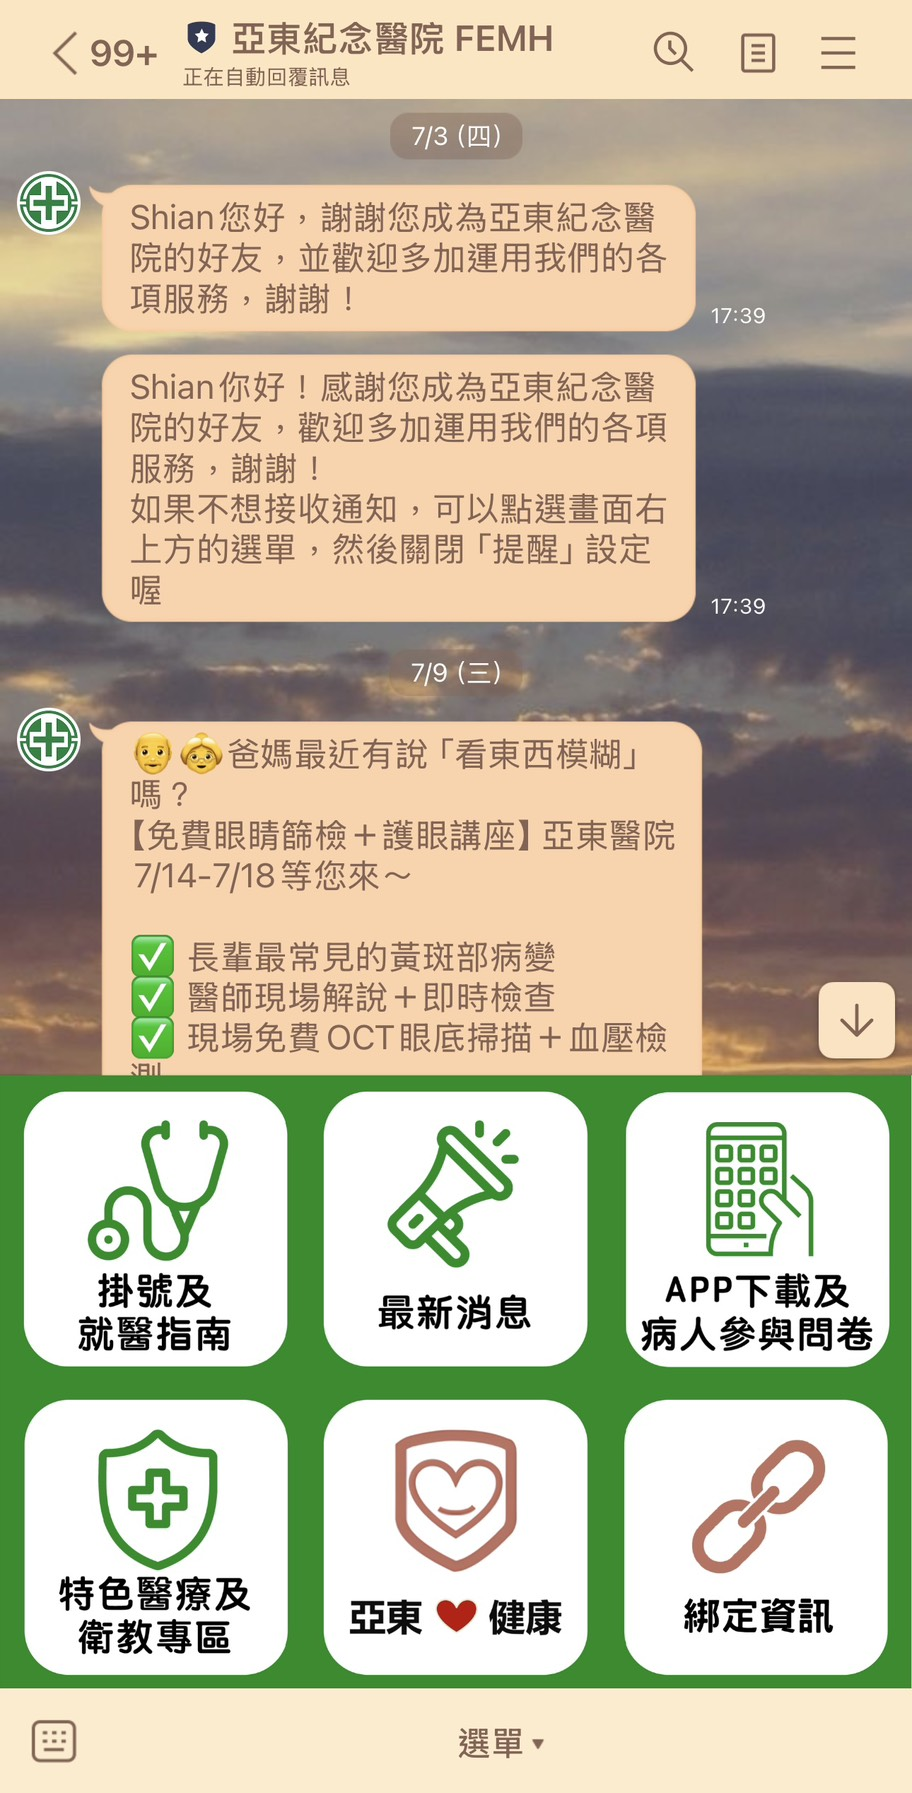
\includegraphics[width=\textwidth]{../../images/line.jpg}
        \caption{Original Chinese interface (source: FEMH LINE official account~\cite{femhline}).}
        \label{fig:line-chinese}
    \end{subfigure}
    \hspace{2cm}
    % right with English
    \begin{subfigure}[t]{0.3\textwidth}
        \centering
        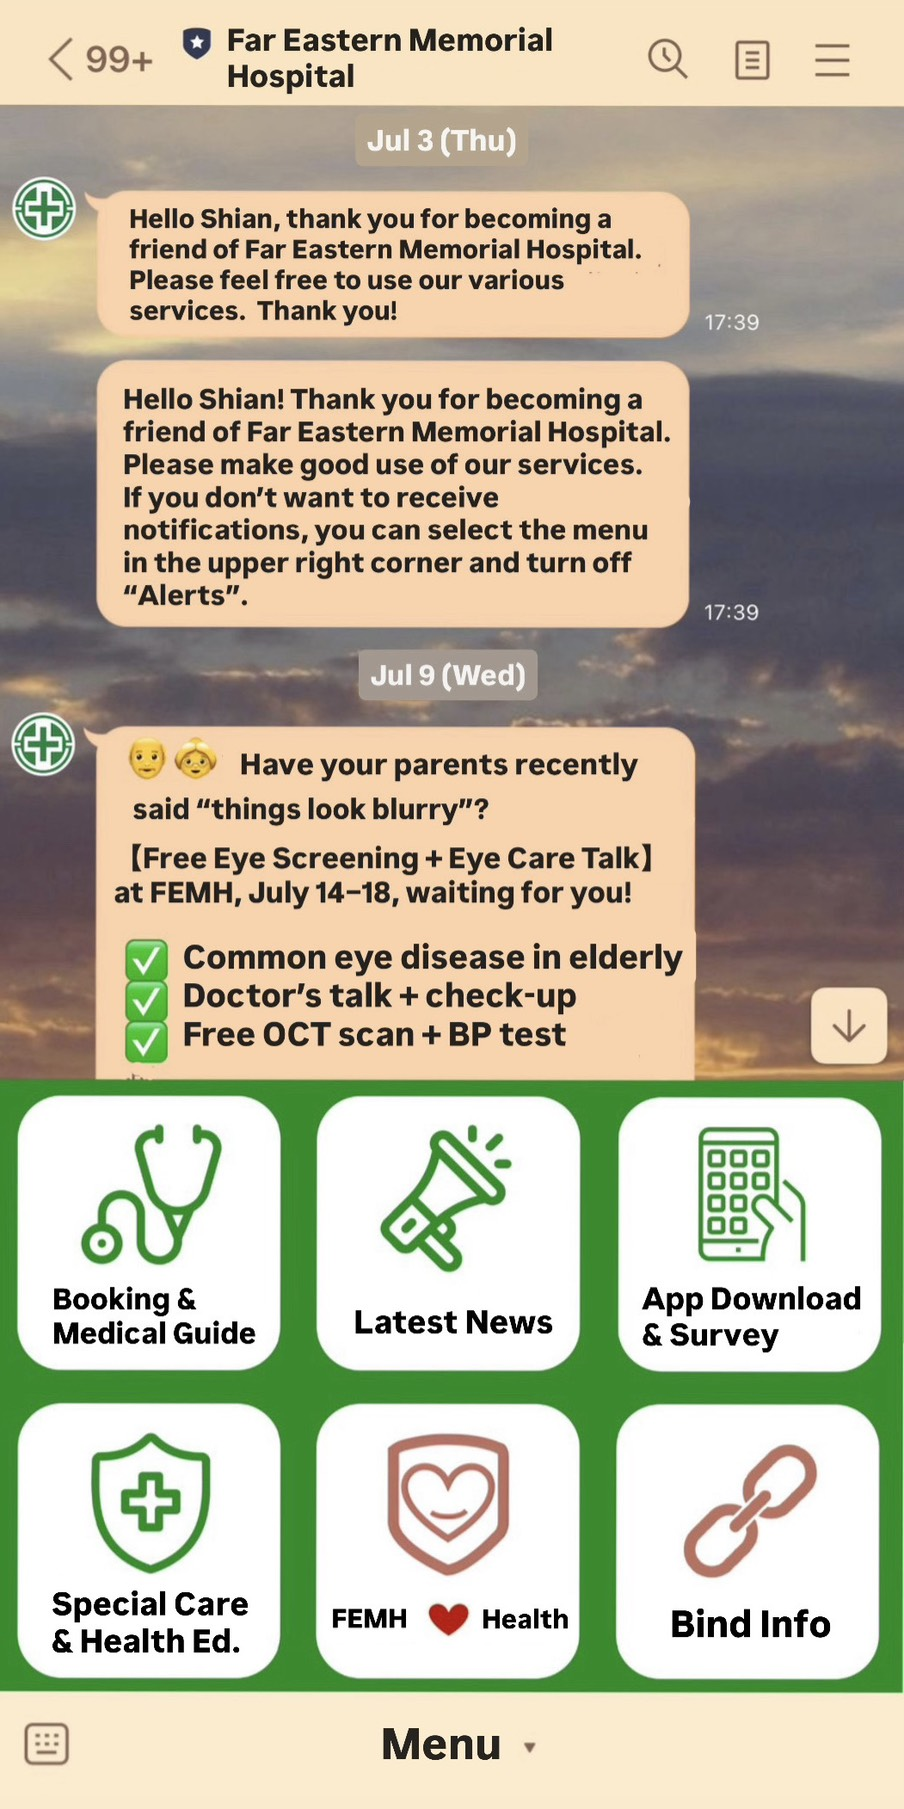
\includegraphics[width=\textwidth]{../../images/line_english.jpg}
        \caption{English translated version (translated by the author, layout unchanged).}
        \label{fig:line-english}
    \end{subfigure}

    \caption{Screenshots of Far Eastern Memorial Hospital (FEMH) LINE services.}
    \label{fig:line-service}
\end{figure}
\noindent

These features are convenient, but each hospital has its own design and menu. Some functions even open in separate websites. There is no unified system, so it can be confusing for some patients, especially older people or those not familiar with technology.


\clearpage


\clearpage
\section{Requirements}
\label{sec:requirements}

This website is aimed at doctors, nurses, and patients to enhance the high performance of clinical flow. This is mainly to reduce the workloads that hospital staff have, and this can also help patients to interact with the doctors using this website. It will provide a number of benefits.

To ensure a functional and effective experience for hospital staff and patients, the system was designed to support a core set of features. These include secure user login and authentication for doctors, nurses, and patients; the ability to record patient vitals and view historical data trends; and an interface for remote consultation to minimise unnecessary hospital visits.

Drawing on the team’s previous experience with similar healthcare platforms, including the Virtual Hospital Africa system, we referenced their approach as a conceptual foundation while adapting the design to our own project scope and requirements.

The system is initially populated with pre-existing mock patient data to facilitate testing and demonstration. In addition to these accounts, the platform supports new patient registration, enabling patients to create their own accounts and access the same core features, including secure login, health query submission, and medical record downloads.

Non-functional requirements include secure authentication with role-based access control, ensuring that only authorised users can access or modify clinical records. This system is stable, operates with fast response, and supports instant workloads. In addition, keep the user interface clear and straightforward to reduce the time that staff have to learn from the system in the hospital. These system capabilities are closely aligned with the user stories presented below.

\vspace{1em}
\begin{table}[H]
\centering
\renewcommand{\arraystretch}{1.4}
\begin{tabular}{|p{2cm}|p{5.2cm}|p{5.2cm}|p{2cm}|}
\hline
\textbf{As a...} & \textbf{I want...} & \textbf{So that...} & \textbf{Technical ability} \\
\hline
Patient & To ask health-related questions online & I can get medical guidance without visiting the hospital & 2--3 \\
\hline
Patient & To download my complete medical record & I can share it with a pharmacy or another healthcare provider & 2--3 \\
\hline
Nurse & To record patient vitals and update profile information & I can ensure accurate data is available for diagnosis & 2--4 \\
\hline
Doctor & To review patient history and vitals trends & I can make informed clinical decisions & 3--5 \\
\hline
Doctor & To add clinical notes and prescriptions & I can provide clear treatment guidance for the patient & 3--5 \\
\hline
\end{tabular}
\caption{Smart Hospital User Stories}
\label{tab:user-stories}
\end{table}
\vspace{1em}
